\documentclass[11pt,a4paper,openany]{article}
\usepackage[french]{babel} % Pacote para traduzir o documento para português
\usepackage[utf8]{inputenc} % Pacote para incluir letras com acentos nos documentos e.g. á, ã, etc; bem como o ç, i.e., c de cedilha, etc
\usepackage[bottom=2cm,top=2cm,left=2cm,right=2cm]{geometry}
\usepackage{amsmath, amssymb} % Pacote para trabalhar com notação matemática
\usepackage{mathtools}
%\usepackage[margin=2cm]{geometry} % Pacote para controlar a margem
\usepackage{graphicx} % Pacote para meter imagens
%\usepackage{subfig} % Pacote para pôr imagens uma ao lado da outra oi gatao
\usepackage[english]{refstyle} % Pacote para referenciar imagens 
\usepackage{float} % o que é isto?? é um pacote  
\usepackage{indentfirst} % mete paragrafo na primeira linha depois de uma section
\usepackage{amsfonts} % alguns símbolos como o Z de numero inteiro
\usepackage{cases} % para os cases
%\usepackage[]{mcode} %usar cOdigo matlab
\usepackage{caption}
\usepackage{subcaption} %figuras lado a lado
%\usepackage{fixltx2e} 
\usepackage{hyperref} 
\usepackage{fancyhdr} %rodape e cabeçalho
\usepackage[export]{adjustbox} %ajustar figuras
\usepackage{graphicx,wrapfig,lipsum} %figuras ao lado do texto
\usepackage{enumerate}
\usepackage{enumitem} %diminuir espaçamento entre item com numeração
\usepackage{circuitikz} %circuitos
\usepackage{titlesec}
\usepackage[T1]{fontenc}
\usepackage{textcomp}
\usepackage{gensymb} %simbolo º
\usepackage{dirtytalk} %aspas \say{}
\usepackage{csquotes}
\usepackage{multirow}
\usepackage{amsmath}
\renewcommand{\thesection}{\arabic{section}} 
\renewcommand{\thesubsection}{\thesection.\arabic{subsection}}
\usepackage{siunitx}
\usepackage{gensymb}
\usepackage{subfiles}
\usepackage{lastpage}
\usepackage{amsmath}
\usepackage{systeme}
\usepackage{comment}

\fancypagestyle{firstpage}{
    \renewcommand{\headrulewidth}{0pt}
    \fancyhead{}
    \cfoot{Page \thepage \hspace{1pt} de \pageref{LastPage}}
}

%% Este lado direito do cabeçalho não me parece bom
\pagestyle{fancy}
\fancyhf{}
\rhead{Simulateur de production et consommation électriques}
\lhead{Informatique}
\cfoot{Page \thepage \hspace{1pt} de \pageref{LastPage}}
\pagenumbering{arabic}

\begin{document}
\thispagestyle{firstpage}

\begin{center}
	\large{
    Informatique\\
    Simulateur de production et consommation électriques \\
    \vspace{10pt}
    \textbf{Notice explicative du code dévéloppé} \\}
    \vspace{10pt}
    DE OLIVEIRA MORENO NEVES, José Afonso \\
\end{center}

Cette petite notice sert à expliquer le code dévéloppé pour la phase individuelle du projet et à montrer les diagrames UML obtenus. Dans le paquetage «executables», j'ai aussi créé 5 classes exécutables simples pour illustrer le comportement des différents éléments du projet. Dans la fin du document, je présente les diagrames UML du projet. Le projet a beaucoup de classes donc je les ai divisé en diagrammes d'accord avec son paquetage.

\subsubsection*{Profiles}

Tout d'abord, j'ai choisi de mettre en œuvre les consommateurs et les producteurs comme les mêmes objets car, du moins à ce stade, ils ne sont caractérisés que par leurs profils de puissance qui sont équivalents. Ensuite, pour pouvoir regrouper des profils implementés par différentes classes, j'ai créé une interface que j'ai appelé «Profile». Si, à l'avenir, des fonctionnalités sont ajoutées au simulateur qui nécessitent la distinction entre producteurs et consommateurs, il faudra modifier cette construction. Cependant, l'interface que j'ai créée peut être utilisée comme un attribut des nouveaux producteurs ou consommateurs.

Pour préciser les profils au long de l'année, j'ai utilisé 3 mécanismes. Tout d'abord, j'ai créé la classe «YearVariation» qui permet de définir un jour de début et un jour de fin d'opération. Deuxièmement, j'ai créé la classe «WeekVariation» qui permet de définir les jours de la semaine où le profil fonctionnera. Troisièmement, j'ai créé l'interface «Parameter» qui permet de créer des paramètres pour chaque profil dont la valeur varie tout au long de l'année. Pour l'instant, j'ai créé deux types de paramètres, constants et sinusoïdaux. Le diagrame UML que réprésente les paramètres est presenté dans la Figure \ref{fig:parameters}.

Pour les variations dans le même jour, j'ai considéré deux types de profiles: les profiles qui durent toute la journée et les profiles qui durent seulement une partie de la journée et qui peuvent se répétir. Les premiers ont une implémentation simple et je présente un exemple dans la classe «DayConstantProfile». Les seconds peuvent en fait représenter les premiers si la durée appropriée est définie et pour eux, je présente trois types différents, constants, linéaires et quadratiques. Pour représenter le fait qu'ils commencent à un certain instant, ont une certaine durée et peuvent être périodiques, j'ai créé la classe «Square» et les ai fait hériter de la classe abstraite «SquaredProfile» qui a un attribut «Square» et les attributs des différentes variations annuelles.

D'autre part, j'ai également défini une classe qui implémente un groupe de profils pour pouvoir représenter différents appareils ou profils composés de différents profils que j'ai nommé «ProfilesGroup». Les classes que j'ai mentioné sont representés dans la Figure \ref{fig:profiles}.

\subsubsection*{Outils de visualisation des résultats}

Jusqu'à présent, j'ai créé deux types d'outils de visualisation de données, une classe pour écrire les données dans un fichier .csv appelée «DataToCSV» et une classe pour afficher des graphiques de puissance, d'énergie et de puissance perdue appelée «DataToPlots». J'ai essayé de rendre simple la création de graphiques de nouvelles quantités en écrivant cette classe. J'ai également défini une interface appelée «DataOutputs» pour les outils de visualisation afin qu'il soit simple d'en ajouter d'autres. Le diagrame correspondent aux outils de visualization est presenté dans la Figure \ref{fig:dataOutputs}.

\subsubsection*{Simulateur}

J'ai également créé un simulateur que j'ai appelé «City», qui reçoit des «ProfileGroups» de producteurs et de consommateurs et des «DataOutputs» et simule la production et la consommation. Il envoie également les résultats à travers la classe «Résultats», presentée dans la Figure \ref{fig:results},  que j'ai définie pour les outils de visualisation, crée un dossier et un fichier dédié à la simulation et applique les outils aux résultats. La classe «City» est representé dans le diagrame de la Figure \ref{fig:city}.

\begin{figure}
    \centering
    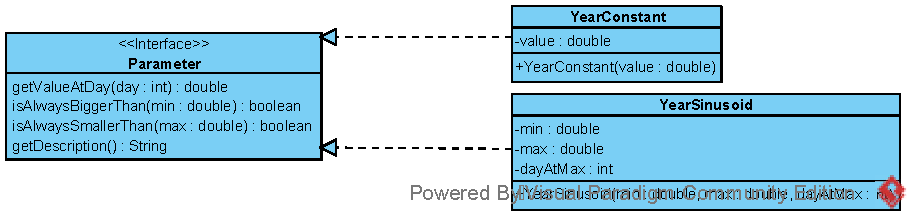
\includegraphics[width = \linewidth]{parameters_cropped.pdf}
    \caption{Diagrame UML associé au paquetage «parameters».}
    \label{fig:parameters}
\end{figure}

\begin{figure}
    \centering
    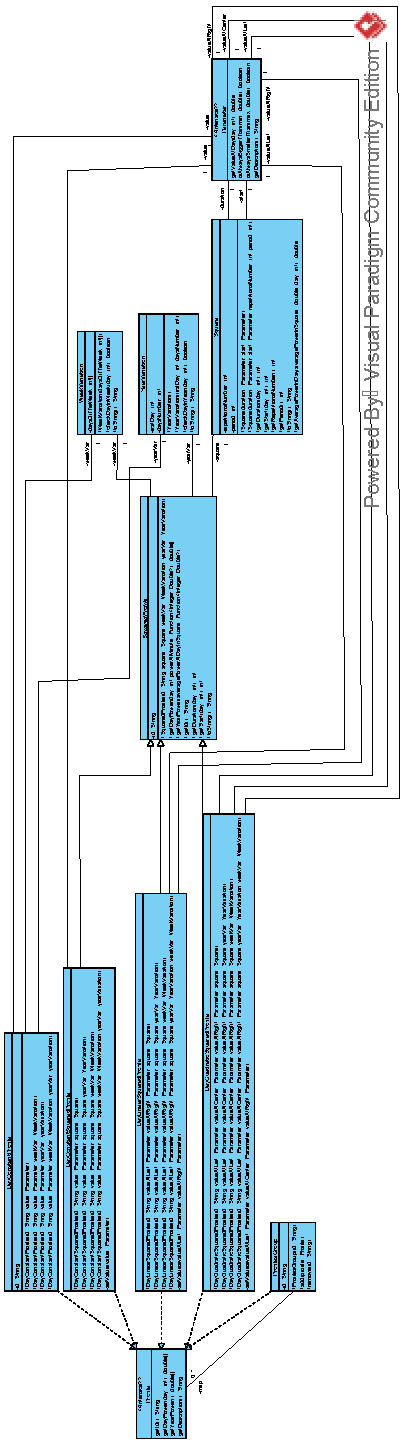
\includegraphics[width = 0.4\linewidth]{profiles_cropped.pdf}
    \caption{Diagrame UML associé au paquetage «profiles».}
    \label{fig:profiles}
\end{figure}

\begin{figure}
    \centering
    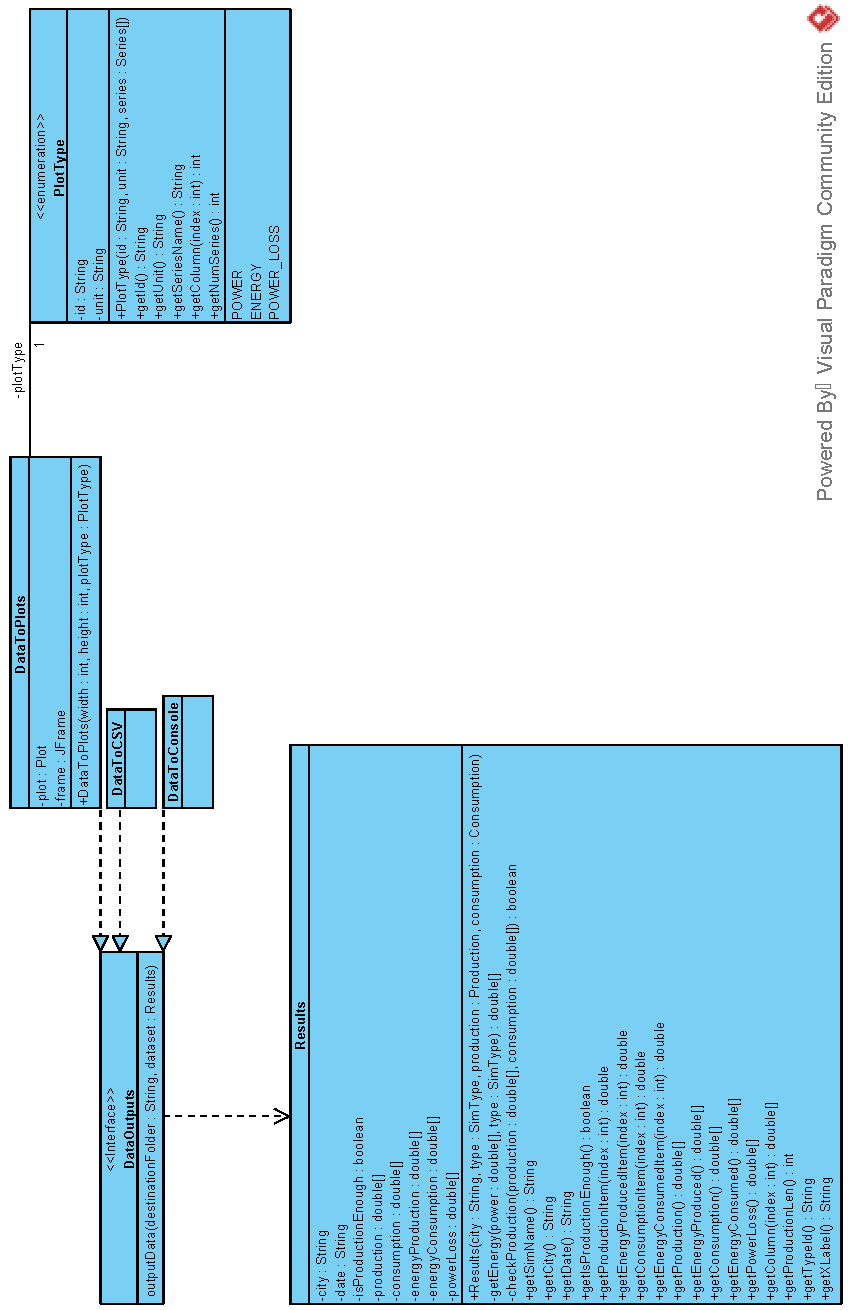
\includegraphics[width = 0.9\linewidth]{dataOutputs_cropped.pdf}
    \caption{Diagrame UML associé au paquetage «dataOutputs».}
    \label{fig:dataOutputs}
\end{figure}

\begin{figure}
    \centering
    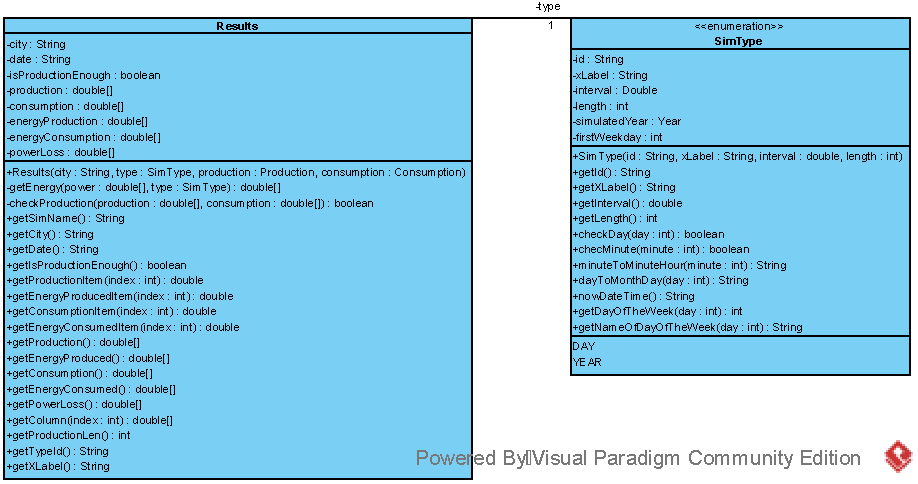
\includegraphics[width = \linewidth]{results_cropped.pdf}
    \caption{Diagrame UML au paquetage «results».}
    \label{fig:results}
\end{figure}

\begin{figure}
    \centering
    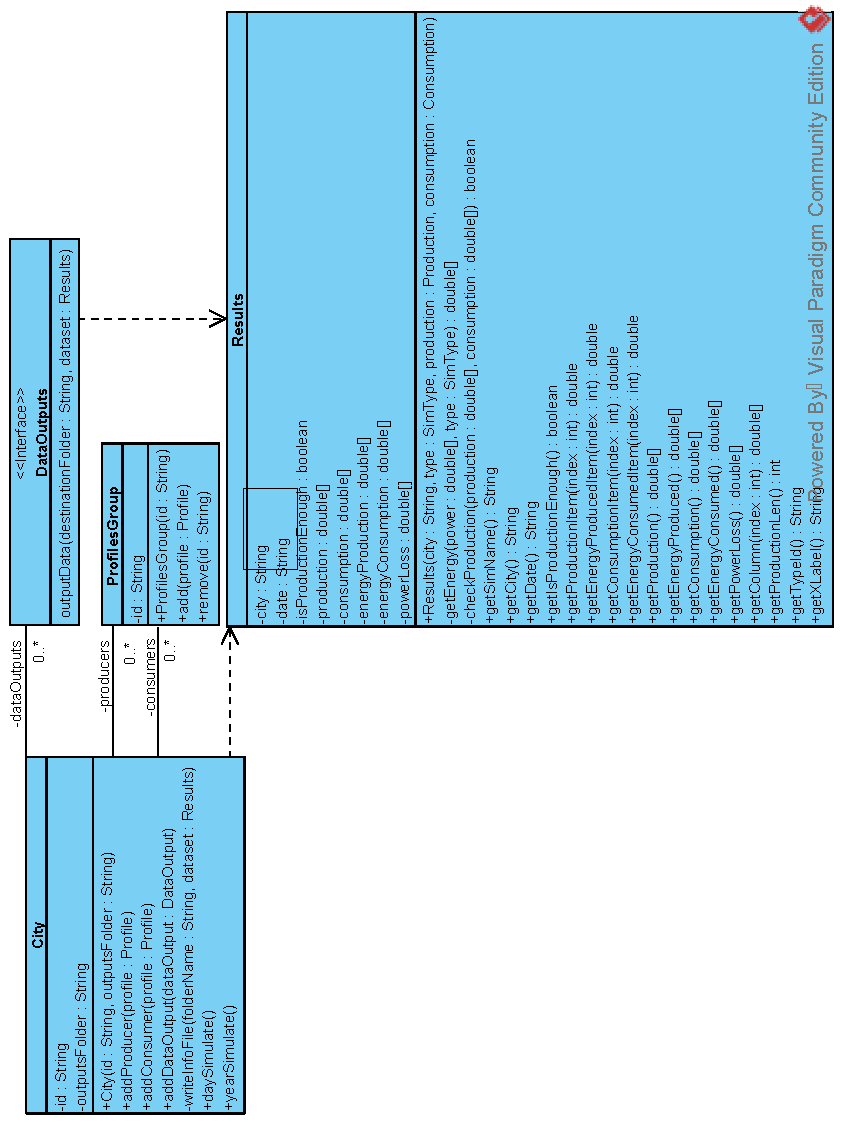
\includegraphics[width = \linewidth]{city_cropped.pdf}
    \caption{Diagrame UML associé à la classe «City».}
    \label{fig:city}
\end{figure}

\end{document}

